\documentclass[a4paper, 11pt, notitlepage, english]{article}

\usepackage{babel}
\usepackage[utf8]{inputenc}
\usepackage[T1]{fontenc, url}
\usepackage{textcomp}
\usepackage{amsmath, amssymb}
\usepackage{amsbsy, amsfonts}
\usepackage{graphicx, color, xcolor}
\usepackage{verbatim, listings, fancyvrb}
\usepackage{parskip}
\usepackage{framed}
\usepackage{amsmath}
\usepackage{multicol}
\usepackage{url}
\usepackage{flafter}
\usepackage{simplewick}
\usepackage{amsthm}
\usepackage{bbold}


\usepackage{caption}
\DeclareCaptionLabelSeparator{colon}{. }
\renewcommand{\captionfont}{\small\sffamily}
\renewcommand{\captionlabelfont}{\bf\sffamily}
\usepackage{float}
%\floatstyle{ruled}
%\restylefloat{figure}
\setlength{\captionmargin}{20pt}
%\addto\captionsenglish{\renewcommand{\figurename}{Fig.}}
\usepackage{bigstrut}
\setlength{\tabcolsep}{12pt}


\newtheorem{theorem}[]{Wick's Theorem}[]

\DeclareUnicodeCharacter{00A0}{~}

\definecolor{javared}{rgb}{0.6,0,0} % for strings
\definecolor{javagreen}{rgb}{0.25,0.5,0.35} % comments
\definecolor{javapurple}{rgb}{0.5,0,0.35} % keywords
\definecolor{javadocblue}{rgb}{0.25,0.35,0.75} % javadoc

\lstset{language=python,
basicstyle=\ttfamily\scriptsize,
keywordstyle=\color{javapurple},%\bfseries,
stringstyle=\color{javared},
commentstyle=\color{javagreen},
morecomment=[s][\color{javadocblue}]{/**}{*/},
morekeywords={super, with},
% numbers=left,
% numberstyle=\tiny\color{black},
stepnumber=2,
numbersep=10pt,
tabsize=2,
showspaces=false,
captionpos=b,
showstringspaces=false,
frame= single,
breaklines=true}

\usepackage{geometry}
\geometry{headheight=0.01mm}
\geometry{top=20mm, bottom=20mm, left=34mm, right=34mm}

\renewcommand{\arraystretch}{2}
\setlength{\tabcolsep}{10pt}
\makeatletter
\renewcommand*\env@matrix[1][*\c@MaxMatrixCols c]{%
  \hskip -\arraycolsep
  \let\@ifnextchar\new@ifnextchar
  \array{#1}}
%
% Definering av egne kommandoer og miljøer
%
\newcommand{\dd}[1]{\ \text{d}#1}
\newcommand{\f}[2]{\frac{#1}{#2}} 
\newcommand{\beq}{\begin{equation}}
\newcommand{\eeq}{\end{equation}}
\newcommand{\bra}[1]{\langle #1|}
\newcommand{\ket}[1]{|#1 \rangle}
\newcommand{\braket}[2]{\langle #1 | #2 \rangle}
\newcommand{\brakket}[2]{\langle #1 || #2 \rangle}
\newcommand{\braup}[1]{\langle #1 \left|\uparrow\rangle\right.}
\newcommand{\bradown}[1]{\langle #1 \left|\downarrow\rangle\right.}
\newcommand{\av}[1]{\left| #1 \right|}
\newcommand{\op}[1]{\hat{#1}}
\newcommand{\braopket}[3]{\langle #1 | {#2} | #3 \rangle}
\newcommand{\ketbra}[2]{\ket{#1}\bra{#2}}
\newcommand{\pp}[1]{\frac{\partial}{\partial #1}}
\newcommand{\ppn}[1]{\frac{\partial^2}{\partial #1^2}}
\newcommand{\up}{\left|\uparrow\rangle\right.}
\newcommand{\upup}{\left|\uparrow\uparrow\rangle\right.}
\newcommand{\down}{\left|\downarrow\rangle\right.}
\newcommand{\downdown}{\left|\downarrow\downarrow\rangle\right.}
\newcommand{\updown}{\left|\uparrow\downarrow\rangle\right.}
\newcommand{\downup}{\left|\downarrow\uparrow\rangle\right.}
\newcommand{\bupup}{\left.\langle\uparrow\uparrow\right|}
\newcommand{\bdowndown}{\left.\langle\downarrow\downarrow\right|}
\newcommand{\bupdown}{\left.\langle\uparrow\downarrow\right|}
\newcommand{\bdownup}{\left.\langle\downarrow\uparrow\right|}
\renewcommand{\d}{{\rm d}}
\newcommand{\Res}[2]{{\rm Res}(#1;#2)}
\newcommand{\To}{\quad\Rightarrow\quad}
\newcommand{\eps}{\epsilon}
\newcommand{\inner}[2]{\langle #1 , #2 \rangle}
\renewcommand{\u}{\uparrow}
\renewcommand{\d}{\downarrow}
\newcommand{\dddd}{\d\d\d\d}
\newcommand{\uddd}{\u\d\d\d}
\newcommand{\dudd}{\d\u\d\d}
\newcommand{\ddud}{\d\d\u\d}
\newcommand{\dddu}{\d\d\d\u}
\newcommand{\uudd}{\u\u\d\d}
\newcommand{\udud}{\u\d\u\d}
\newcommand{\uddu}{\u\d\d\u}
\newcommand{\duud}{\d\u\u\d}
\newcommand{\dudu}{\d\u\d\u}
\newcommand{\dduu}{\d\d\u\u}
\newcommand{\uuud}{\u\u\u\d}
\newcommand{\uudu}{\u\u\d\u}
\newcommand{\uduu}{\u\d\u\u}
\newcommand{\duuu}{\d\u\u\u}
\newcommand{\uuuu}{\u\u\u\u}
\newcommand{\m}{\text{-}}
\newcommand{\ui}{{\u_1}}
\newcommand{\uii}{{\u_2}}
\newcommand{\uiii}{{\u_3}}
\newcommand{\di}{{\d_1}}
\newcommand{\dii}{{\d_2}}
\newcommand{\diii}{{\d_3}}

\newenvironment{psmallmatrix}
  {\left(\begin{smallmatrix}}
  {\end{smallmatrix}\right)}

\newenvironment{bsmallmatrix}
  {\left[\begin{smallmatrix}}
  {\end{smallmatrix}\right]}



\newcommand{\bt}[1]{\boldsymbol{#1}}
\newcommand{\mat}[1]{\textsf{\textbf{#1}}}
\newcommand{\I}{\boldsymbol{\mathcal{I}}}
\newcommand{\p}{\partial}
%
% Navn og tittel
%
\author{Jonas van den Brink \\ \texttt{j.v.brink@fys.uio.no}}
\title{First Midterm Project \\ FYS-KJM4480}

\begin{document}
\maketitle

In this project we will be looking at two simple models for the ground state of the helium and beryllium atoms, with two and four electrons respectively. We use the hydrogenic wavefunctions as our single-particle wavefunctions throughout.

\subsection*{The System}
Any atom is characterized by its atomic number $Z$, which denotes how many protons are in the atomic core. Any element corresponds to atoms with a given atomic number, helium having $Z=2$ and beryllium having $Z=4$. A charge neutral atom will have the same number of electrons as the number of protons in its core. An atom that has more or less electrons than protons is ionized and is therefore electrically charged.

As the nucleus is much more massive than the electrons, and they have electric charge of equal magnitude, it is reasonable to assume that the motion of the electrons will be much more pronounced than that of the core. In fact, it is quite reasonable to say the core is purely stationary. This approximation is known as the \emph{Born-Oppenheimer} approximation. It reduces the complexity of our equations significantly, as we now only have to solve for the wave-function of the electrons.

Under the Born-Oppenheimer approximation, the Schrödinger equation can be solved in closed form for the hydrogen atom. However, for the helium atom and heavier atoms, this is no longer possible due to the Coloumb interaction between the electrons. We can however find \emph{hydrogenic} wave-functions. These hydrogen-like wave-functions are the wave-functions describing a nucelus with atomic number $Z$, but with only a single electron attached to it. When more electrons are added, these hydrogenic wave-functions are no longer stationary states for the system, they do however form an orthonormal basis in which the new stationary states can be expanded.

The hydrogenic wavefunctions have quantum numbers $n, l$ and $m_l$. And as electrons are fermions with spin $s=1/2$, we know that we have a double spin degeneracy for each hydrogenic wavefunction. So our system has single-particle states with quantum numbers $n, l, m_l, s, m_s$.

Excluding fine-structure, the Hamiltonian for an atom with atomic number $Z$ and $N$ electrons is given (in atomic units) by
$$\op{H} = \sum_{i=1}^N\op{h}_0(x_i) + \sum_{i<j}^N \frac{1}{r_{ij}},$$
where $\op{h}_0(x_i) = \op{t}(x_i) - Z/r_i.$

We won't actually use the explicit form of the hydrogenic wave-functions, nor the Hamiltonian in this project. Instead we realize that the Hamiltonian is a sum of a one-body operator and a two-body operator and write it as
$$\op{H} = \sum_{i=1}^N \op{h}_0(x_1) + \sum_{i<j}^N \op{h}_1(x_1,x_2).$$
The only time the explicit form of these onebody and twobody operators is of interest is when we need to calculate the matrix elements
$$\braopket{\alpha}{\op{h}_0}{\beta}, \qquad \braopket{\alpha\beta}{\op{h}_1}{\gamma\delta},$$
where $\alpha,\beta,\gamma$ and $\delta$ are our hydrogenic single-particle wave-functions. Instead of calculating the onebody matrix elements explicitly, we will use the result
$$\braopket{\alpha}{\op{h}_0}{\beta} = -\frac{Z^2}{2n^2}\delta_{\alpha\beta}.$$
For the two-body matrix elements, we realize that they are given by a combination of a spatial integral and a spin integral. We now look further into what this means for the values of the two-body matrix elements.

\section*{Spin Summation} \label{sec:spin}

When looking at the matrix element $\braopket{pq}{\op{v}}{rs}$, we remember that it is shorthand for the integral
$$\braopket{pq}{\op{v}}{rs} = \iint \psi^*_p(x_1)\psi^*_q(x_2)\op{v}(x_1,x_2)\psi_r(x_1) \psi_s(x_2) \ \mbox{d} x_1 \mbox{d} x_2.$$
In our case however, the wavefunction consists of both a spatial and a spin part. As our Hamiltonian doesn't affect the spin part of the wave-function, we can split our integral into a radial integral and a spin integral 
$$\braopket{p_{\chi_1}q_{\chi_2}}{\op{v}}{r_{\chi_3} s_{\chi_4}} = \braopket{pq}{\op{v}}{rs}\braket{\chi_1\chi_2}{\chi_3\chi_4}.$$
The radial integral can be computed analytically for $s$-waves, and we have recieved a tabulated list of these matrix elements, so they can be considered known. The spin integral can easily be computed from the fact that the spin-orbitals are orthonormal, so we have
$$\braket{\chi_1\chi_2}{\chi_3\chi_4} = \braket{\chi_1}{\chi_3}\braket{\chi_2}{\chi_4} = \delta_{\chi_1\chi_3}\delta_{\chi_2\chi_4}.$$
So we see that if both particles have the same spin, the spin integral becomes unity, and in all other cases the spin integral vanishes and takes the radial integral with it. 

Let us now look closer at what this means for the antisymmetrized matrix elements of the twobody operator. Keeping only the terms where the spins are equal, we get
\begin{align*}
\brakket{p_\u q_\u}{r_\u s_\u}	&= \brakket{p_\d q_\d}{r_\d s_\d} = \braopket{pq}{\op{v}}{rs} - \braopket{pq}{\op{v}}{sr}, \\
\brakket{p_\u q_\d}{r_\u s_\d}	&= \brakket{p_\d q_\u}{r_\d s_\u} = \braopket{pq}{\op{v}}{rs}, \\
\brakket{p_\u q_\d}{r_\d s_\u}	&= \brakket{p_\d q_\u}{r_\u s_\d} = -\braopket{pq}{\op{v}}{sr}, \\
\brakket{p_\u q_\u}{r_\u s_\d}	&= \brakket{p_\u q_\u}{r_\d s_\u} = \brakket{p_\u q_\d}{r_\u s_\u} = \brakket{p_\d q_\u}{r_\u s_\u} = 0, \\
\brakket{p_\u q_\d}{r_\d s_\d}	&= \brakket{p_\d q_\u}{r_\d s_\d} = \brakket{p_\d q_\d}{r_\u s_\d} = \brakket{p_\d q_\d}{r_\d s_\u} = 0, \\
\brakket{p_\u q_\u}{r_\d s_\d}	&= \brakket{p_\d q_\d}{r_\u s_\u} = 0.
\end{align*}
So we see that out of 16 possible combinations, 10 vanish completely, 2 only have the direct term, 2 only have the exchange term and only two terms have both the direct and exchange term. The spin summation simplifies things considerably.

\clearpage

\section*{Exercise 1a)}
We start of by looking at the helium atom, meaning we have two electrons in our system. We will look at the single-particle states and create an ansatz for the ground state and singly-excited states.

\subsubsection*{Single-particle states}
For our single-particle states, we use the hydrogenic wave-functions. We limit ourselves to the $s$-waves $1s$-$3s$, meaning $l=0$ and $n\leq3$. It follows from this that $m_l = 0$. We also know that $s=1/2$ for electrons, so $m_s = \pm 1/2$. With these limitations, there are then six linearily independant single-particle states that acts as our basis for the possible single-particle states of the system. 

We could label these single-particle states as $\ket{n l m_l s m_s}$, but we would rather use something simpler as the only quantum numbers that actually change are $n$ and $m_s$. We therefore use the notation $\ket{n_\u}$ for the $m_s=1/2$ states and $\ket{n_\d}$ for the $m_s=-1/2$ states. Using this notation, our single-particle basis is
$$\{1_\u, 1_\d, 2_\u, 2_\d, 3_\u, 3_\d \}.$$
This set of single-particle states is orthonormal and any single-particle state in our system can be written as a linear combination of these basis-states. We will however limit ourselves to states where the total spin project $M_S$ is zero, meaning the two electrons in the system have opposite spins.

\subsubsection*{An ansatz for the ground state}

We would now like to construct an ansatz for the ground state. The single-particle states are the hydrogenic wave-functions, meaning they are the solution of the onebody part of the Hamiltonian. For the hydrogenic wavefunctions the energies are known and increase with $n$. Therefore, if there was no interaction between the electrons, the ground-state would be constructed from the states $\ket{1_\u}$ and $\ket{1_\d}$. 

Now, when interaction \emph{is} included, this is no longer the true ground state. However, the ground-state without interaction is a good starting point, and so we will use this state as our ansatz for the ground state. 

Due to electrons being indistinguishable and fermions, we must construct a Slater determinant to describe the two-particle system. In first quantization, our ansatz can then be written
$$\ket{\Phi_0} = \frac{1}{\sqrt{2}}\big(\ket{1_\u}\ket{1_\d} - \ket{1_\d}\ket{1_\u}\big).$$
In second quantization however, we don't have to explicitly express the anti-symmetry of the wavefunction algebraicly. Instead we construct the ground state from the true vacuum, so we have
$$\ket{\Phi_0} = \op{a}_{1_\u}^\dagger\op{a}_{1_\d}^\dagger\ket{0}.$$

\clearpage

\subsubsection*{The Fermi-vacuum and hole-formulation\footnote{Much of the text from this section is taken from the exercises from week 4, where I gave motivation for the formulation and went into detail about the reference vacuum, pseduo creation- and annihilation operators and looked at the general Wick's theorem.}}
In second quantization we described a system by denoting all the occupied single-particle states. When doing any useful calculation we collapse our state into a string of creation operators working on the true vacuum. We can however, introduce a reference state to take the place of the true vacuum, this reference state is usally referred to as either the \emph{core} or the \emph{Fermi-vacuum}.

To collapse a general state into a string of operators acting on the Fermi-vacuum generally requires the use of \emph{both} creation and annihilation operators. For example, if we let $\ket{0}$ denote the true vacuum, and define our reference state to be $\ket{ijk}$, then we can collapse a given state as follows
$$\ket{abijk} = \op{a}_a^\dag\op{a}_b^\dag\op{a}_i^\dag\op{a}_j^\dag\op{a}_k^\dag\ket{0}, \qquad \ket{abijk} = \op{a}_a^\dag\op{a}_b^\dag\ket{ijk} = \op{a}_a^\dag\op{a}_b^\dag\ket{\Phi_0},$$
where we have denoted the Fermi-vacuum by $\ket{\Phi_0}$, which in this case contained the single-particle states $i, j$ and $k$.

Any annihilation operator destroys the true vacuum state. For the Fermi-vacuum however, the given single-particle state might be contained in the reference, in which case the vacuum is \emph{not} destroyed---but it will now contain a \emph{hole}. Holes are simply vacant states in the reference vacuum. So we have
$$\op{\alpha} \ket{0} = 0, \qquad \op{\alpha} \ket{\Phi_0} = \begin{cases}
	\ket{\Phi_\alpha} \mbox{ if } \alpha \in \Phi_0, \\
	0 \mbox{ if } \alpha \not\in \Phi_0, \\
\end{cases}$$
where $\Phi_\alpha$ denotes the vacuum-state with the state $\ket{\alpha}$ removed. However, remembering wich states are and aren't contained in the \emph{Fermi}-vacuum becomes tiring, so we want to introduce notation that makes it easy to see this at all times. We turn to the notation introduced in Shavitt and Bartlett, where we let $a, b, c,\ldots$ denote states \emph{not} in the reference and $i,j,k, \ldots$ be states in the reference. The states $p,q,r,\ldots$ can be used if a general state is needed. We can then for any general reference vacuum write
$$\op{i}^\dag \ket{\Phi_0} = 0, \qquad \bra{\Phi_0} \op{i} = 0, \qquad \op{a}\ket{\Phi_0} = 0, \qquad \bra{\Phi_0}\op{a}^\dag = 0.$$

A given physical system often has a constant number of particles, so states like $\ket{\Phi_i}$ with just a particle removed, are often not intersting. Those that are interesting, are states like $\ket{\Phi_i^a}$. Here, a particle that was below the Fermi-level has been removed, leaving a hole, while a particle above the Fermi-level has been added. This one-particle-one-hole state is easily interpret as a state where a single particle has been excited when compared to the reference vacuum.

If we now let the ground state of the system be the reference vacuum, we can easily create single-excited states by looking at the possible one-particle-one-hole states, and doubly-excited states by looking at two-particle-two-hole states and so on.

\clearpage

\subsubsection*{Excited states for the helium atom}
Now, we don't know the true ground state for the helium atom, but we have found an ansatz for the ground state, so we let this be our reference state that defines the Fermi-vacuum. Meaning 
$$\ket{\Phi_0} = \op{a}_{1_\u}^\dagger\op{a}_{1_\d}^\dagger\ket{0},$$
now denotes the Fermi vacuum. We will look at all the possible one-particle-one-hole and two-particle-two-hole excitations from this Fermi vacuum under the restriction that $M_s$ is preserved and zero.

The possible one-particle-one-hole states are
\begin{align*}
\ket{\Phi_{1_\u}^{2_\u}} &= \op{a}_{2_\u}^\dagger \op{a}_{1_\u} \ket{\Phi_0}, \qquad\qquad
\ket{\Phi_{1_\u}^{3_\u}} = \op{a}_{3_\u}^\dagger \op{a}_{1_\u} \ket{\Phi_0}, \\
\ket{\Phi_{1_\d}^{2_\d}} &= \op{a}_{2_\d}^\dagger \op{a}_{1_\d} \ket{\Phi_0}, 
\qquad\qquad
\ket{\Phi_{1_\d}^{3_\d}} = \op{a}_{3_\d}^\dagger \op{a}_{1_\d} \ket{\Phi_0}.
\end{align*}
And the possible two-particle-two-hole states are
\begin{align*}
\ket{\Phi_{1_\u1_\d}^{2_\u2_\d}} &= \op{a}_{2_\u}^\dagger \op{a}_{2_\d}^\dagger \op{a}_{1_\u} \op{a}_{1_\d} \ket{\Phi_0}, \\
\ket{\Phi_{1_\u1_\d}^{2_\u3_\d}} &= \op{a}_{2_\u}^\dagger \op{a}_{3_\d}^\dagger \op{a}_{1_\u} \op{a}_{1_\d} \ket{\Phi_0}, \\
\ket{\Phi_{1_\u1_\d}^{3_\u2_\d}} &= \op{a}_{3_\u}^\dagger \op{a}_{2_\d}^\dagger \op{a}_{1_\u} \op{a}_{1_\d} \ket{\Phi_0}, \\
\ket{\Phi_{1_\u1_\d}^{3_\u3_\d}} &= \op{a}_{3_\u}^\dagger \op{a}_{3_\d}^\dagger \op{a}_{1_\u} \op{a}_{1_\d} \ket{\Phi_0}.
\end{align*}

All the states we have construced is illustrated in figure \ref{fig:1a}.


\begin{figure}[bhpt]
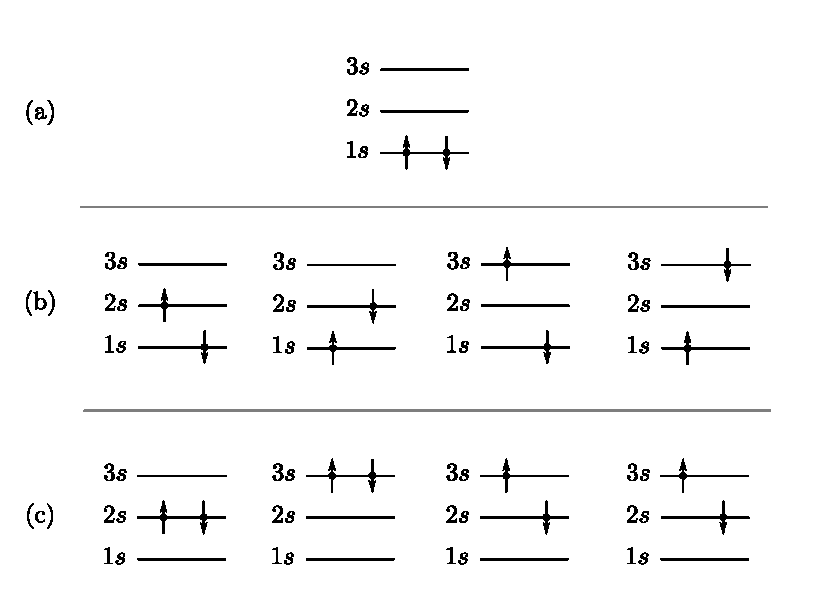
\includegraphics{project1a.pdf}
\caption{Schematic of states built from the hydrogenic single-particle states in the helium atom with two electrons. \textbf{(a)} The ansatz for the ground state, i.e., the Fermi-vacuum. \textbf{(b)} Single-excited states from the Fermi-vacuum, i.e., one-particle-one-hole states. \text{(c)} Doubly-excited states, i.e., two-particle-two-hole states. \label{fig:1a}}	
\end{figure}

\clearpage

\section*{Exercise 1b)}
We will now define our Hamiltonian in second quantization, so that we can compute the reference energy for the ansatz ground state as a function of the atomic number. 

\subsubsection*{Hamiltonian in second quantization}

In second quantization, general onebody and twobody operators can be written
\begin{align*}
\op{T} &= \sum_{pq} \braopket{p}{\op{t}}{q} \op{a}_p^\dagger \op{a}_q, \\
\op{V} &= \sum_{pqrs} \braopket{pq}{\op{v}}{rs} \op{a}_p^\dagger\op{a}_q^\dagger \op{a}_r \op{a}_s,
\end{align*}
note that we use $p,q,r,s$ to denote the states as operators generally work on both states below and above the Fermi vacuum. Using Wick's theorem, we can rewrite these operators to\footnote{See the problem set for week 4.}
\begin{align*}
\op{T} &= \sum_{pq} \braopket{p}{\op{t}}{q} \{\op{a}_p^\dagger \op{a}_q\} + \sum_i \braopket{i}{\op{t}}{i}, \\
\op{V} &= \frac{1}{4}\sum_{pqrs} \brakket{pq}{rs} \{\op{a}_p^\dag \op{a}_q^\dag \op{a}_s\op{a}_r\} + \sum_{pqi} \brakket{pi}{qi} \{ \op{a}_p^\dag \op{a}_q \} + \frac{1}{2}\sum_{ij} \brakket{ij}{ij}.
\end{align*}
Using this, we can write the Hamiltonian for our system out in second quantization as
\begin{align*}
\op{H} &= \sum_{pq} \braopket{p}{\op{h}_0}{q} \{\op{a}_p^\dagger \op{a}_q\} + \frac{1}{4}\sum_{pqrs} \brakket{pq}{rs}\{\op{a}_p^\dag \op{a}_q^\dag \op{a}_s\op{a}_r\} \\ &\qquad+ \sum_i \braopket{i}{\op{h}_0}{i} + \sum_{pqi} \brakket{pi}{qi} \{ \op{a}_p^\dag \op{a}_q \} + \frac{1}{2}\sum_{ij} \brakket{ij}{ij},
\end{align*}
where $\op{h}_0 = \op{t}_0 - Z/r$ and $\op{h}_1 = 1/r_{ij}$.

\subsubsection*{Finding the reference energy}
We now want to find the reference energy, which is the expectation value of our ansatz ground state. This is by definition given by
$$E[\Phi_0] = \braopket{\Phi_0}{\op{H}}{\Phi_0}.$$
Any normal-product vanishes when acting on the Fermi vacuum, so we are only left with the two terms of the Hamiltonian where there is no normal-product
$$E[\Phi_0] = \braopket{\Phi_0}{\op{H}}{\Phi_0} = \sum_{i}\braopket{i}{\op{h}_0}{i} + \frac{1}{2}\sum_{ij} \brakket{ij}{ij}.$$
As expected, we are left with summing only over the single-particle states below the Fermi-level. In our case, we have the single-particles states
$$\{1_\u, 1_\d, 2_\u, 2_\d, 3_\u, 3_\d \},$$
where the first two are below the Fermi-level, and the rest are above it.

\clearpage

Writing out the sums we then get
\begin{align*}
E[\Phi_0] &= \braopket{1_\u}{\op{h}_0}{1_\u} + \braopket{1_\d}{\op{h}_0}{1_\d} \\ &\qquad + \frac{1}{2}\big(\brakket{1_\u1_\u}{1_\u1_\u} + \brakket{1_\u1_\d}{1_\u1_\d} + \brakket{1_\d1_\u}{1_\d1_\u} + \brakket{1_\d1_\d}{1_\d1_\d}\big).
\end{align*}
We now use spin summations. We see that the first and last terms give both the direct and exchange terms, while the two middle terms only contribute the direct term. In this case, the direct term and the exchange term cancel out, so we are left with 
\begin{align*}
E[\Phi_0] &= 2\braopket{1}{\op{h}_0}{1} + \braopket{11}{\op{v}}{11}.
\end{align*}
We know that the one-body element is given by 
$$\braopket{i}{\op{h}_0}{j} = -\frac{Z^2}{2n^2}\delta_{ij},$$
and the value of the element $\braopket{11}{\op{v}}{11}$ is tabulated. We have then found the reference energy as a function of $Z$
$$E[\Phi_0](Z) = \frac{5}{8}Z - Z^2.$$
Inserting for the atomic number of helium, $Z=2$, we get the reference energy
$$E[\Phi_0] = -2.75.$$
The true ground state has an energy of $-2.9037$ with our Hamiltonian. We see that our reference energy, which is derived from our simple ansatz for the ground state is surprisingly close to the real ground state, with a relative error of only 5.3\%. Note that it should come as no surprise that our reference energy is above the true ground state energy as this is predicted by the variational principle.

\section*{Exercise 1c)}

We now limit our system even further and only allow single-excited states beyond the Fermi-level. We use these Slater-determinants as a basis and find the linear combination that gives a minimum in the energy.

\subsubsection*{The basis and hamiltonian matrix}

Our state basis is now given by the Fermi-vacuum and the four possible one-particle-one-hole excitations, so we have the basis
$$\{\ket{\Phi_0}, \ket{\Phi_\di^\uii}, \ket{\Phi_\ui^\uiii}, \ket{\Phi_\di^\dii}, \ket{\Phi_\di^\diii}\}.$$
This basis spans a five-dimensional Hilbert space. We can represent any operator, including the Hamiltonian, as a five-by-five matrix in this space. We start of by using closure on the operator
$$\op{H} = \sum_{pq} \ket{p}\braopket{p}{\op{H}}{q}\bra{q}.$$
We now define the matrix representation of the operator by stating that the matrix element is given by
$$H_{pq} = \braopket{p}{\op{H}}{q}.$$
And we can now interpret an operator working on a state as a matrix-vector product, if we let the state be given as a coefficient-vector in the same basis
$$\ket{i}_p = \braket{p}{i} = \sum_q \braopket{p}{\op{H}}{q} \braket{q}{j} = \sum_p H_{pq}\ket{j}_q.$$
Solving the Schrödinger equation then reduces to finding the eigenvectors and eigenvalues of the Hamiltonian matrix.

\subsubsection*{General expressions for the matrix elements}
To find the Hamiltonian matrix of our system we must compute the matrix elements $H_{pq}$ where $p$ and $q$ are the Slater determinants in our basis, i.e., we are looking at computing the elements
$$\braopket{\Phi_0}{\op{H}}{\Phi_i^a}, \qquad \braopket{\Phi_i^a}{\op{H}}{\Phi_j^b},$$
where 
$$i, j \in \{1_\u, 1_\d\} \mbox{ and } a, b \in \{2_\u, 2_\d, 3_\u, 3_\d \}.$$

Using diagrammatic form, the first matrix element can be written
\begin{center}

\includegraphics{project1c_1}
\end{center}
This is a Hugenholtz diagram (as opposed to a Goldstone diagram), meaning the final term is asymmetrized. We can write this diagram out algebraicly as
$$\braopket{\Phi_0}{\op{H}}{\Phi_i^a} = \braopket{a}{\op{h}_0}{i} + \sum_{k} \brakket{ak}{ik}.$$
The matrix element for two one-particle-one-hole states is generally given by
\begin{center}
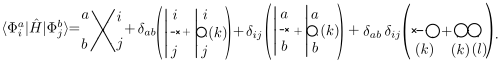
\includegraphics{project1c_2}
\end{center}
These are again Hugenholtz-diagrams, so we can write it out algebraicly as
\begin{align*}
\braopket{\Phi_i^a}{\op{H}}{\Phi_j^b} &= \brakket{aj}{ib} -\delta_{ab}\bigg(\braopket{i}{\op{h}_0}{j} + \sum_{k} \brakket{ik}{jk}\bigg) + \delta_{ij}\bigg(\braopket{a}{\op{h}_0}{b} + \sum_{k} \brakket{ak}{bk}\bigg) \\
&\qquad\qquad + \delta_{ab}\delta_{ij}\bigg(\sum_{k} \braopket{k}{\op{h}_0}{k} + \frac{1}{2}\sum_{kl}\brakket{kl}{kl}\bigg).
\end{align*}
Note that if there are two non-coincicdences between the SDs we only get one term, from the twobody operator, but if there is only one non-coincidence or none we also get contributions from the onebody operator, as well as more contributions from the twobody operator. The factor 1/2 for the final term is read out from the diagram from the redundancy in the $k$ and $l$ indices, see Shavitt and Bartlett chapter 4 for more info on diagrammatic notation.

\subsubsection*{Symmetry in the Hamiltonian matrix}
As the Hamiltonian matrix is a five-by-five matrix, there are 25 elements we need to compute. However, there is a lot of symmetry in the matrix which we can exploit to simplify the work.

First of, the Hamiltonian matrix must be hermitian, meaning the transpose elements must be complex conjugates of each other, and as our elements are purely real we have
$$
\braopket{\Phi_0}{\op{H}}{\Phi_i^a} = \braopket{\Phi_i^a}{\op{H}}{\Phi_0},
$$
this means we only have to calculate half of the off-diagonal terms.
Secondly, as the Hamiltonian does not affect the spin-orbital of the wavefunctions, we see that elements with completely opposite spins must be equal
$$\braopket{\Phi_0}{\op{H}}{\Phi_{1_\d}^{n_\d}} = \braopket{\Phi_0}{\op{H}}{\Phi_{1_\u}^{n_\u}} \mbox{  and  } \braopket{\Phi_{1_\u}^{n_\u}}{\op{H}}{\Phi_{1_\u}^{m_\u}} = \braopket{\Phi_{1_\d}^{n_\d}}{\op{H}}{\Phi_{1_\d}^{m_\d}}.$$

\subsubsection*{Calculating the matrix elements}
We are now ready to calculate the matrix elements of the Hamiltonian matrix. This can of course be done by hand, but that is a lot of work. As we already have full expressions for each matrix element, we can can calculate the Hamiltonian matrix symbollically on a computer. 

The matrices are computed symbollically, but inserting for $Z=2$ for the helium atom gives the Hamiltonian matrix
\begin{align*}
H = \begin{pmatrix}
-2.750 &  0.179 &  0.179 &  0.088 &  0.088 \\
0.179 &  -2.080 &  0.044 &  0.101 &  0.022 \\
0.179 &  0.044 &  -2.080 &  0.022 &  0.101 \\
0.088 &  0.101 &  0.022 &  -2.023 &  0.012 \\
0.088 &  0.022 &  0.101 &  0.012 &  -2.023 \\	
\end{pmatrix}.
\end{align*}
We can clearly see the symmetries in the Hamiltonian matrix, as it is symmetric about the main diagonal due to all elements being purely real. We also see that elements with completely opposite spins are equal as a result of spin degeneracy.

\subsubsection*{Finding the eigenvalues and eigenvectors}
Now that we have represented the Hamiltonian as a matrix, we can write the Schrödinger equation out as an eigenvalue matrix problem
$$H\vec{v}_k = \eps_k\vec{v}_k.$$
Where $\vec{v}_k$ is the k'th eigenvector and $\eps_k$ is the k'th eigenvalue. As these are eigenvectors and eigenvalues of the Hamiltonian, they are in fact the coefficient-vectors of the stationary states and their corresponding energies. The smallest eigenvalue is therefore the ground state energy in the given Hilbert space.

We now compute the eigenvalues of the Hamiltonian using numerical tools and find them to be
\begin{align*}
\lambda_1 &= -2.83864845, \\
\lambda_2 &= -2.16988063, \\
\lambda_3 &= -2.13619337, \\
\lambda_4 &= -1.98904529, \\
\lambda_5 &= -1.82322132. 
\end{align*}
The lowest eigenvalue is the approximation to the ground state energi, so we have found
$$E = -2.8386.$$
Now, this is still an approximation to the exact ground state energy, as we severally limited our Hilbert space by having a basis consisting of only 5 SDs, which were in turn constructed from a very limited set of single-particle states.

This method for finding the ground state energy also obeys the variational principle, so again we were sure that the approximation would overshoot the exact energy. As our ansatz ground state is part of our basis, we also knew that this approximation should be at least equally good to the last one, and probably better. So we knew theoretically that we needed to land between the exact energy and the previous approximation, which we did
$$E_{\rm exact} = -2.9037 \leq E = -2.8386 \leq E[\Phi_0] = -2.750,$$
this is then at least a small confirmation that our calculations have been correct. Our new approximation has a relative error of 2.2\%, which again is surprisingly good considering how limited our basis actually is. It is also quite a bit better than the previous approximation which was given by the expectation value for the energy of the pure ansatz ground state.

\subsection*{Exercise 1d)}
So far we have only looked at the helium atom, we will now look at the beryllium atom in the same manner. The beryllium atom has atomic number $Z=4$, and so has four electrons. 

\subsection*{Single-particle states, Slater determinants and a basis}
As before, we use the hydrogenic wave-functions as our single-particle states. As the hydrogenic wave-functions already is built on the assumption of no interaction between the electrons, they are not affected by the fact that we have more electrons in the beryllium atom than in the helium atom. They are however slightly affected by the fact that beryllium has a higher atomic number $Z$, and so the coloumb interaction with the atomic core is stronger for every electron. We use the same limitations on the single-particle states as earlier, looking only at the $s$-waves for $n\leq 3$. So we have the quantum numbers $n=1,2,3$, $l=m_l=0$, $s=1/2$ and $m_s=\pm 1/2$. We therefore use the same notation as earlier.

Due to spin degeneracy, each $s$-level can inhabit two electrons. The ansatz for the ground state is then two electrons in $1s$ and two electrons in two $2s$---as earlier, this is the state that has the lowest energy \emph{if} we disregard interaction between the electrons. In second quantization, the ground state can then be written
$$\ket{\Phi_0} = \op{a}_{1_\u}^\dagger\op{a}_{1_\d}^\dagger\op{a}_{2_\u}^\dagger\op{a}_{2_\d}^\dagger \ket{0}.$$
We let this be our Fermi-vacuum. We can now create four one-particle-one-hole states if we enforce $M_s = 0$. These are
\begin{align*}
\ket{\Phi_{1_\u}^{3_\u}} &= \op{a}_{3_\u}^\dagger \op{a}_{1_\u} \ket{\Phi_0}, \qquad\qquad
\ket{\Phi_{1_\d}^{3_\d}} = \op{a}_{3_\d}^\dagger \op{a}_{1_\d} \ket{\Phi_0}, \\
\ket{\Phi_{2_\u}^{3_\u}} &= \op{a}_{3_\u}^\dagger \op{a}_{2_\u} \ket{\Phi_0}, 
\qquad\qquad
\ket{\Phi_{2_\d}^{3_\d}} = \op{a}_{3_\d}^\dagger \op{a}_{2_\d} \ket{\Phi_0}.
\end{align*}
These states are illustrated in figure \ref{fig:1d}, shown on the next page

\begin{figure}[thbp]
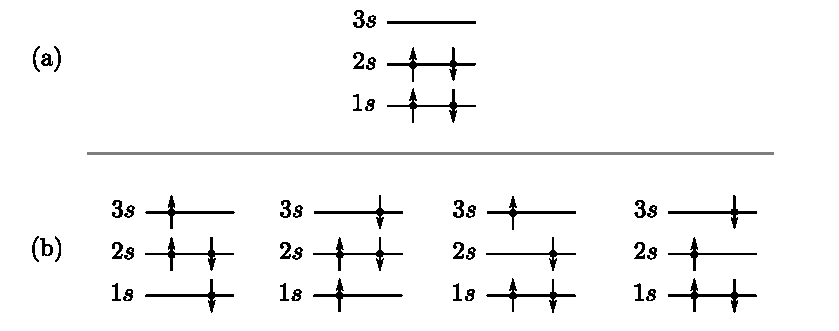
\includegraphics{project1d.pdf}
\caption{Schematic of states built from the hydrogenic single-particle states in the beryllium atom with four electrons. \textbf{(a)} The ansatz for the ground state, i.e., the Fermi-vacuum. \textbf{(b)} Single-excited states from the Fermi-vacuum, i.e., one-particle-one-hole states. \label{fig:1d}}	
\end{figure}

\newpage

\subsection*{Calculating the reference energy}
The reference energy of the beryllium ansatz ground state is given by
\begin{align*}
E[\Phi_0] &= \braopket{\Phi_0}{\op{H}}{\Phi_0} = \sum_{i}\braopket{i}{\op{h}_0}{i} + \frac{1}{2}\sum_{ij} \brakket{ij}{ij},
\end{align*}
where $i,j\in\{1_\u,1_\d,2_\u,2_\d\}$. Writing out the sums gives
\begin{align*}
E[\Phi_0] &= 2\braopket{1}{\op{h}_0}{1} + 2\braopket{2}{\op{h}_0}{2} + \frac{1}{2}\big(
\brakket{1_\u 1_\u}{1_\u 1_\u} + \brakket{1_\u 1_\d}{1_\u 1_\d} 
+ \brakket{1_\u 2_\u}{1_\u 2_\u} \\&\quad
+ \brakket{1_\u 2_\d}{1_\u 2_\d}  
+ \brakket{1_\d 1_\u}{1_\d 1_\u}  
+ \brakket{1_\d 1_\d}{1_\d 1_\d}  
+ \brakket{1_\d 2_\u}{1_\d 2_\u}  
\\&\quad
+ \brakket{1_\d 2_\d}{1_\d 2_\d}  
+ \brakket{2_\u 1_\u}{2_\u 1_\u}  
+ \brakket{2_\u 1_\d}{2_\u 1_\d}  
+ \brakket{2_\u 2_\u}{2_\u 2_\u}  
\\&\quad
+ \brakket{2_\u 2_\d}{2_\u 2_\d}  
+ \brakket{2_\d 1_\u}{2_\d 1_\u}  
+ \brakket{2_\d 1_\d}{2_\d 1_\d}  
+ \brakket{2_\d 2_\u}{2_\d 2_\u}  
\\&\quad
+ \brakket{2_\d 2_\d}{2_\d 2_\d}\big). \\[-0.8cm]
\end{align*}
We immediately see that
$$\brakket{1_\u 1_\u}{1_\u 1_\u} = \brakket{1_\d 1_\d}{1_\d 1_\d} = \brakket{2_\u 2_\u}{2_\u 2_\u} =  \brakket{2_\d 2_\d}{2_\d 2_\d} = 0,$$
Using this and all the other spin summations, we end up with 
\begin{align*}
E[\Phi_0] = 2\braopket{1}{\op{h}_0}{1} + 2\braopket{2}{\op{h}_0}{2} + 
\braopket{11}{\op{v}}{11} + 4\braopket{12}{\op{v}}{12} - 2\braopket{12}{\op{v}}{21} + \braopket{22}{\op{v}}{22}.
\end{align*}
Inserting for alle the matrix elements gives
\begin{align*}
E[\Phi_0](Z) = \frac{586373}{373248}Z - \frac{5}{4}Z^2.
\end{align*}
Inserting for berylliums atomic number, $Z=4$, gives the reference energy
$$E[\Phi_0] = -13.7160.$$
The exact energy is $-14.6674$ which means we have a relative error of 6.5\%, which is ever so slightly larger than for the helium atom, but still surprisingly good. Note that the variational principle is also apparent here, as the approximation overshoots the exact energy.

\subsubsection*{Constructing the Hamiltonian matrix}
Again we limit the system to the ansatz ground state and the four one-particle-one-hole Slater determinants, meaning we have the basis
$$ \{ \ket{\Phi_0}, \ket{\Phi_\di^\diii}, \ket{\Phi_\ui^\uiii}, \ket{\Phi_\dii^\diii}, \ket{\Phi_\uii^\uiii} \}.$$
We construct the Hamiltonian in the same manner as we did for the helium atom in exercise 1c. The main difference is that we have four electrons in our system, meaning
$$i,j,k,l \in \{1_\u, 1_\d, 2_\u, 2_\d\}, \qquad a,b \in \{3_\u, 3_\d\}.$$
We can use the exact same expressions for the onebody and twobody operators as we used in exercise 1c. In our program, we only have to alter $N$ and $Z$ to four, and redefine our SD basis.

Running the program gives the hamiltonian matrix
\begin{align*}
H = \begin{pmatrix}
-13.716 &  0.189 &  0.189 &  0.445 &  0.445  \\
0.189 &  -9.655 &  0.023 &  -0.393 &  0.008  \\
0.189 &  0.023 &  -9.655 &  0.008 &  -0.393  \\
0.445 &  -0.393 &  0.008 &  -13.688 &  0.030  \\
0.445 &  0.008 &  -0.393 &  0.030 &  -13.688 	
\end{pmatrix}.
\end{align*}

\subsubsection*{Eigenvalues of the Hamiltonian}
Using numpy, we find the eigenvalues of the hamiltonian matrix for the beryllium atom to be
\begin{align*}
\lambda_1 &= -14.36210798, \\
\lambda_2 &= -13.7577963, \\
\lambda_3 &= -13.05941173, \\
\lambda_4 &= -9.63871331, \\
\lambda_5 &= -9.58503496. 
\end{align*}
As before, the lowest of these is our approximation to the groun state energy, so
$$E = -14.3621.$$
Again we see that, as expected, the new approximation lies between the ansatz ground state reference energy and the exact energy
$$E_{\rm exact} = -14.6674 \leq E = -14.3621 \leq E[\Phi_0] = -13.7160.$$ 
The new approximation has a relative error of 2.1\%, which unlike the ansatz ground state reference energy, is actually better than for the helium atom!






\clearpage

\section*{Exercise 1e)}
We now turn to a new method to find a new approximation to the ground state energy, the Hartree-Fock method. This method aims to find the single best Slater determinant to approximate the ground state. 

\subsubsection*{Change-of-basis}
We can change from one single-particle basis to another by doing a unitary transform. Any state $\psi_p$ can be expanding in the basis $\{\phi_\lambda\}$ as follows
$$\psi_p = \sum_\lambda C_{p\lambda} \phi_\lambda,$$
where $C_{p\lambda}$ is a matrix element in the unitary matrix $C$. If the original basis is orthonormal, then any basis we change into is also orthonormal.

\subsubsection*{The Hartree-Fock equations}
We want to approximate the ground state of the system by a single Slater determinant. The idea is therefore rather simple, we write out the reference energy with respect to a general Slater determinant. By expanding that SD into a new basis, we can minimize the reference energy with respect to the coefficients of that expansion. Finding the Slater determinant that best approximates the ground state then reduces to a minimization problem.

We start of by writing out the reference energy of a general Slater determinant
$$E = \braopket{\Phi}{\op{H}}{\Phi} = \sum_{p=1}^N \braopket{p}{\op{h}_0}{p} + \frac{1}{2}\sum_{p=1}^N\sum_{q=1}^N\braket{pq|}{pq}.$$
Expanding the states into a new basis gives us 
$$E = \sum_{p=1}^N \sum_{\alpha \beta} C^*_{p \alpha} C_{p \beta}\braopket{\alpha}{\op{h}_0}{\beta} + \frac{1}{2}\sum_{p=1}^N\sum_{q=1}^N\sum_{\alpha\beta\gamma\delta} C_{p\alpha}^* C_{q \beta}^* C_{p \gamma} C_{q \delta} \braket{\alpha\beta|}{\gamma\delta}.$$
We then want to find a minimum in the reference energy with respect to the coefficients. A necessary condition for a minimum is that the variation $\delta E$ is zero. This is not a sufficient condition, as there might be maxima and saddle points.

The minimization problem is not without constraints, as we do require that the single-particle wave-functions are orthogonal and the transformation unitary. As $C$ is unitary, we know that
$C^\dagger C = \mathbb{1}$, so we have
$$\sum_\alpha C_{a \alpha}^* C_{a \alpha} = (C^\dagger C)_{a \alpha} = \delta_{a \alpha}.$$
This is the case for any $a$, so we can state the constraints on the problem as
$$\bigg(\sum_\alpha C_{a\alpha}^* C_{a\alpha} = (C^\dagger C)_{a\alpha} - \delta_{a\alpha}\bigg) = 0 \qquad \forall \ a.$$
This set of $N$ constraints can be included in the minimization process through the use of Lagrangian multipliers. As each constraint is equal to zero, we can multiply it by a constant $\eps_a$ and freely add it to the energy without changing anything
$$E = E - \sum_a \eps_a \bigg(\sum_\alpha C_{a \alpha}^* C_{a \alpha} - \delta_{a\alpha}\bigg).$$

We can then find the variation in the reference energy. From the definition we find
$$\delta E = \sum_{k\alpha}\frac{\p E}{\p C_{k\alpha}^*} \delta C_{k\alpha}^* + \sum_{k\alpha} \frac{\p E}{\p C_{k\alpha}}\delta C_{k\alpha} - \sum_{k\alpha}\eps_k (C_{k\alpha} \delta C_{k\alpha}^* + C_{k\alpha}^*\delta C_{k\alpha}.) .$$
Each coefficient $C_{p\alpha}$ and $C_{p\alpha}^*$  is independant, and so can be varied independantly. For a minimum, we know that $\delta E = 0$ for all possible variations in coefficients, and so $\delta E = 0$ gives rise to a set of equations, one for each coefficient:
$$\delta E = 0 \quad \Rightarrow \quad \bigg(\frac{\p E}{\p C_{k\alpha}^*} - \eps_k C_{k\alpha} \bigg)\delta C_{k\alpha}^* = 0 \quad \forall \quad k, \alpha,$$
which is satisfied if and only if
$$\frac{\p E}{\p C_{k\alpha}^*} - \eps_k C_{k\alpha} = 0 \ \forall\ k, \alpha.$$
When we take the derivative of the original energy with respect to a specific coefficient, we get
$$\sum_{\beta} C_{k \beta}\braopket{\alpha}{\op{h}_0}{\beta} + \sum_{p=1}^N \sum_{\beta\gamma\delta} C_{p\beta}^* C_{k \gamma} C_{p \delta} \braket{\alpha\beta|}{\gamma\delta} - \eps_k C_{k\alpha} = 0.$$
As $\beta$ and $\gamma$ are simply dummy variables we can relabel them, giving
$$\sum_\gamma \bigg(\braopket{\alpha}{\op{h}_0}{\gamma} + \sum_{p=1}^N\sum_{\beta\delta} C_{p\beta}^* C_{p \delta} \braket{\alpha\beta|}{\gamma\delta}\bigg)C_{k \gamma} - \eps_k C_{k\alpha} = 0 \quad \forall \ k, \alpha.$$
We defined the expression in the parenthensis as the Hartree-Fock operator\footnote{More accurately, the expression the parenthensis is the $\alpha\gamma$ matrix element of the matrix representation of the Hartree-fock operator in the original basis.}, which we denote with $\op{h}_{\alpha\gamma}^{\rm HF}$. We can then write our necessary condition for minimizing the energy as
$$\sum_\gamma \op{h}_{\alpha\gamma}^{\rm HF}C_{k\gamma} = \eps_{k} C_{k\alpha} \quad \forall \ k, \alpha.,$$
which are the Hartree-Fock equations. We see that we can interpret the left-hand side as a matrix-vector product, so we can write
$$h^{\rm HF} \mathbf{C}_k = \eps_k \mathbf{C}_k,$$
where $h^{\rm HF}$ is the Hartree Fock operator represented in the original basis, and $\mathbf{C}_k$ is the coefficient-vector of the $k$'th eigenvector of the Hartree-Fock operator, and $\eps_k$ is its eigenvalue. The eigenvalue corresponds to the single-particle energy of the new state.

\clearpage

\section*{Exercise 1f)}
We will now construct the Hartree-Fock matrix using the single particle states $1s$-$3s$ with spin degeneracy for both the helium and beryllium atoms. We then have
$$\alpha, \gamma \in \{1_\u, 1_\d, 2_\u, 2_\d, 3_\u, 3_\d \},$$
meaning the Hartree-Fock matrix will be a 6-by-6 matrix. 

\subsubsection*{Assembling the Hartree-Fock matrix}
To assemble the HF matrix, we need to know the matrix $C$. When solving the HF equations iteratively, we use the solution from the previous timestep to assemble the new HF matrix. For the first iteration, we must then make a guess of the matrix $C$, normally we set it equal to the identity matrix, meaning the coefficients are $C_{\alpha\beta} = \delta_{\alpha\beta}$. 

To assemble the matrix, we use a python script that computes the elements from the formula
\begin{align*}
h_{\alpha\gamma}^{\rm HF} &= \braopket{\alpha}{\op{h}_0}{\gamma} + \sum_{p=1}^N\sum_{\beta\delta} C_{p\beta}^* C_{p \delta} \braket{\alpha\beta|}{\gamma\delta}
\end{align*}
This expression is valid for both the helium and beryllium atoms, but they will of course have a different $N$ and $Z$ value. Calculating all the matrix elements gives the two following matrices
\begin{align*}
h^{\rm HF}_{\rm helium} =
	\begin{pmatrix}
-0.750 &  0 &  0.179 &  0 &  0.088 &  0   \\
0 &  -0.750 &  0 &  0.179 &  0 &  0.088   \\
0.179 &  0 &  0.296 &  0 &  0.180 &  0   \\
0 &  0.179 &  0 &  0.296 &  0 &  0.180   \\
0.088 &  0 &  0.180 &  0 &  0.164 &  0   \\
0 &  0.088 &  0 &  0.180 &  0 &  0.164   
\end{pmatrix}
\end{align*}
\begin{align*}
h^{\rm HF}_{\rm beryllium} =
	\begin{pmatrix}
-3.909 &  0 &  0.392 &  0 &  0.189 &  0   \\
0 &  -3.909 &  0 &  0.392 &  0 &  0.189   \\
0.392 &  0 &  0.193 &  0 &  0.445 &  0   \\
0 &  0.392 &  0 &  0.193 &  0 &  0.445   \\
0.189 &  0 &  0.445 &  0 &  0.527 &  0   \\
0 &  0.189 &  0 &  0.445 &  0 &  0.527   
	\end{pmatrix}
\end{align*}

\clearpage

\subsubsection*{Solving the HF equations}
Now that we have found the HF matrices for both helium and beryllium, we can solve the HF equations. The HF equations could be written as the matrix-vector equation
$$h^{\rm HF} \mat{C}_k = \eps_k \mat{C}_k,$$
so solving the equations means finding the eigenvectors and corresponding eigenvalues of the HF matrix. We do this numerically. 

For helium we find the new single-particle energies
$$\lambda_1 = \lambda_2 = 0.3577, \qquad \lambda_3=\lambda_4 = 0.4925 \qquad \lambda_5 = \lambda_6 = 1.1182,$$
and for beryllium they are
$$\lambda_1 = \lambda_2 = -3.1825, \qquad \lambda_3=\lambda_4 = 0.3546 \qquad \lambda_5 = \lambda_6 = 1.3204.$$
In both cases, we see that there are three distinct eigenvalues each occuring twice. This isn't a big surprise, as we have double spin degeneracy in our single-particle states, but the Hamiltonian makes no dinstinction of spin. 

Note that we have listed our eigenvalues in increasing order, this is vitally important for the success of the algorithm, as we are summing over the $N$ first states. If we want to find the ground state energy, we need to sum over the $N$ lowest energy states. As we are using numpy.linalg.eig, which is a wrapper for the LAPACK eig, we need to explicitly order the coefficient matrix in this manner after finding it before progressing with our computations.

We also get coefficient matrices for both helium and beryllium, but we won't list them here.

\subsubsection*{Calculating the ground state energy}
Now that we have solved the HF eigenvalue equations, we can calculate the approximate ground state energy from the formula
$$E = \sum_{p=1}^N \sum_{\alpha \beta} C^*_{p \alpha} C_{p \beta}\braopket{\alpha}{\op{h}_0}{\beta} + \frac{1}{2}\sum_{p=1}^N\sum_{q=1}^N\sum_{\alpha\beta\gamma\delta} C_{p\alpha}^* C_{q \beta}^* C_{p \gamma} C_{q \delta} \braket{\alpha\beta|}{\gamma\delta},$$
which you might recall was the expression for the energy of a general Slater determinant of $N$ particles---this formula was the basis for the entire HF method.

When we compute the resulting energies, using the coefficient matrices we found in the last section for helium and beryllium, we find that the resulting approximations to the ground state energies are
\begin{align*}
E_{\rm helium} &= -2.8354, \\
E_{\rm beryllium} &= -14.6551.
\end{align*}
We see that both values are above the exact energy, which is good, or we would have broken the variational principle and something would definitly be wrong. We also see that the values we found lie below the energies we found for the ansatz ground states. This isn't very surprising as the ansatz ground state is a single SD, and the HF-method aims to find the single SD with the lowest energy, we therefore expect the HF-method to find a better SD than the one we simply guessed at.


\clearpage

\section*{Exercise 1f)}
\subsubsection*{The Algorithm}
We now perform the Hartree-Fock minimization iteratively. The algorithm can be sketched as follows
\begin{enumerate}
	\item Make some guess for the coefficient matrix $C$.
	\item Assemble $h_{HF}$ from the coefficient matrix $C$.
	\item Find the eigenvectors of $h_{HF}$ and order them correctly. These then form the new coefficient matrix $C$.
	\item Repeat steps 2 and 3 until some tolerance is met.
	\item Calculate the energy resulting from the final coefficient matrix.
\end{enumerate}
There are different possibilities for the tolerance criterion. One posibility is looking at the single-particle energies we get from the eigenvalues of $h_{HF}$. If these change very little from one iteration to the next, we have most likely reached a convergence. Another possibility is looking at the energy itself.

We need to guess at a coefficient matrix to start the iterative scheme. In the previous exercise we started by using a diagonal matrix for $C$, other possibilities is letting it simply be zero or we could let it be random. We implement all these in our code, so that we can test if they all converge to the same solution.

\subsubsection*{The Code}
The full code is attached in an appendix at the end of the project.

\subsubsection*{Results} 
The program converges to the same solution for all three methods for the inital $C$ for both atoms. The program converges to the following values.
\begin{align*}
E_{\rm helium} &= -2.8311, \\
E_{\rm beryllium} &= -14.5091.
\end{align*}
We first note that the variational principle is still fulfilled. Next we note that even though the method converges to a specific value, it is not the exact value, one might wonder why. The answer is that the method converges to the best single Slater determinant that approximates the ground state energy. As the true ground state energy might be a linear combination of several SDs, the method cannot actually reach the exact energy.


\clearpage

\section*{Summary}

In this project we set out with the goal of finding the ground state energy of the helium and beryllium atoms. This energy cannot be found in closed-form due to the electron-electron interaction so we are left hoping to find good approximations. We had knowledge of the exact energy for our system, meaning we could compare our approximations to the exact solution throughout.

We used the hydrogenic wave-functions as our single-particle states. We imposed limitations on these single-particle states, giving us a small basis of single-particle states. To describe our system of two and four electrons, we constructed Slater determinants from these states.

First we calculated the energy of the Slater determinant that would have been the ground states of the system if we had no electron-electron interaction. This method is incredibly simple, and had surprisingly good results, having a relative error of only 5-6\%.

Next we defined a set of one-particle-one-holde Slater determinants in addition to our ansatz ground state. We then had 5 SDs spanning a five-dimensional Hilbert space. By representing our Hamiltonian as a matrix in this space, we could find the linear combination of these SDs that gave the lowest possible energy, which was next approximation to the ground state. This method involved some more computations, but was still quite simple and intuitive. We ended up with a relative error of about 2\%, which is really good for such a simple approximation method.

Next we turned to the Hartree-Fock method. By writing out the energy expectancy of a general SD, we could expand the single-particle states of that SD into our hydrogenic wavefunction basis. This gave us an expression for the energy which was only dependant on the coefficients. We then treated the problem like a minimization problem, finding the coefficients that produced the SD that minimized the energy of the system. 

Finally we performed the Hartree-Fock method iteratively, repeating the minimization problem. The method converged to a specific energy, independant of what intial guess we used for the coefficient matrix $C$. Altough the method converged, it did not reach the exact energy, as it is simply the best single Slater determinant energy, which might be a good enough approximation of the exact solution.

\begin{table}[h!]
\caption{Full table of results.}
\centering
\begin{tabular}{l||l|l|l|l|l}
Helium & Ansatz GS & 5xSD basis & 1 it. HF & Conv. HF & Exact \\ \hline\hline
E [a.units] & -2.7500 & -2.8386 & -2.8354 & -2.8311 & -2.9037 \\
Rel. error & 5.3\% & 2.2\% & 2.5\% & 2.2\% & 
\\ \hline\hline
\end{tabular}

\vspace{1cm}

\begin{tabular}{l||l|l|l|l|l}
Beryllium & Ansatz GS & 5xSD basis & 1 it. HF & Conv. HF & Exact \\ \hline\hline
E [a.units] & -13.7160 & -14.3621 & -14.6551 & -14.5091 & -14.6674 \\
Rel. error & 6.5\% & 2.1\% & 0.1\% & 1.1\% & 
\\ \hline\hline
\end{tabular}
\end{table}

\clearpage

\section*{Appendix A - Code for Hartree-Fock solver}
\lstinputlisting{1f.py}



% Writing out the sum over $\beta$, we have
% \begin{align*}
% h_{\alpha\gamma}^{\rm HF} &= \braopket{\alpha}{\op{h}_0}{\gamma} + \brakket{\alpha1}{\gamma1} + \brakket{\alpha\overline{1}}{\gamma\overline{1}} + \brakket{\alpha2}{\gamma2} + \brakket{\alpha\overline{2}}{\gamma\overline{2}} + \brakket{\alpha3}{\gamma3} + \brakket{\alpha\overline{3}}{\gamma\overline{3}}.
% \end{align*}
% Due to spin summation, we now see that all matrix elements where $\alpha$ and $\gamma$ have opposite spins vanish. For the elements where $\alpha$ and $\gamma$ have the same spin, we see that every pair of terms with the same $n$ will contribute two direct terms and one exchange term. This means that the matrix elements with the same $n$-level will be the same, independant of spin, we therefore now use the letters $i$ and $j$ to denote the $n$-level. We can then write
% \begin{align*}
% h_{ij}^{\rm HF} &= 
% \braopket{i}{\op{h}_0}{j} + 2\braopket{i 1}{\op{v}}{j 1} - \braopket{i 1}{\op{v}}{1 j} + 2\braopket{i 2}{\op{v}}{j 2} - \braopket{i 2}{\op{v}}{2 j} \\ &\qquad+ 2\braopket{i 3}{\op{v}}{j 3} - \braopket{i 3}{\op{v}}{3 j} 
% \end{align*}
% We can now insert for $i, j \in \{1,2,3\}$. Using
% $$\braopket{i}{\op{h}_0}{j},$$
% we see that only the diagonal terms has any contribution from the onebody operator due to orthogonality of the wavefunction. The diagonal terms become
% \begin{align*}
% h_{11}^{\rm HF} &= -\frac{Z^2}{2} + \braopket{1 1}{\op{v}}{1 1}  + 2\braopket{1 2}{\op{v}}{1 2} - \braopket{1 2}{\op{v}}{2 1} + 2\braopket{1 3}{\op{v}}{1 3} - \braopket{1 3}{\op{v}}{3 1}, \\
% h_{22}^{\rm HF} &= 
% -\frac{Z^2}{8} + 2\braopket{2 1}{\op{v}}{2 1} - \braopket{2 1}{\op{v}}{1 2} + \braopket{2 2}{\op{v}}{2 2}  + 2\braopket{2 3}{\op{v}}{2 3} - \braopket{2 3}{\op{v}}{3 2}, \\
% h_{33}^{\rm HF} &= 
% -\frac{Z^2}{18} + 2\braopket{3 1}{\op{v}}{3 1} - \braopket{3 1}{\op{v}}{1 3} + 2\braopket{3 2}{\op{v}}{3 2} - \braopket{3 2}{\op{v}}{2 3} + \braopket{3 3}{\op{v}}{3 3} . 
% \end{align*}
% The non-diagonal terms get no contribution from the onebody operator and so are
% \begin{align*}
% h_{12}^{\rm HF} &= 
% 2\braopket{1 1}{\op{v}}{2 1} - \braopket{1 1}{\op{v}}{1 2} + 2\braopket{1 2}{\op{v}}{2 2} - \braopket{1 2}{\op{v}}{2 2} + 2\braopket{1 3}{\op{v}}{2 3} - \braopket{1 3}{\op{v}}{3 2}, \\
% h_{13}^{\rm HF} &= 
% 2\braopket{1 1}{\op{v}}{3 1} - \braopket{1 1}{\op{v}}{1 3} + 2\braopket{1 2}{\op{v}}{3 2} - \braopket{1 2}{\op{v}}{2 3} + 2\braopket{1 3}{\op{v}}{3 3} - \braopket{1 3}{\op{v}}{3 3}, \\
% h_{21}^{\rm HF} &= 
% 2\braopket{2 1}{\op{v}}{1 1} - \braopket{2 1}{\op{v}}{1 1} + 2\braopket{2 2}{\op{v}}{1 2} - \braopket{2 2}{\op{v}}{2 1} + 2\braopket{2 3}{\op{v}}{1 3} - \braopket{2 3}{\op{v}}{3 1}, \\
% h_{23}^{\rm HF} &= 
% 2\braopket{2 1}{\op{v}}{3 1} - \braopket{2 1}{\op{v}}{1 3} + 2\braopket{2 2}{\op{v}}{3 2} - \braopket{2 2}{\op{v}}{2 3} + 2\braopket{2 3}{\op{v}}{3 3} - \braopket{2 3}{\op{v}}{3 3}, \\
% h_{31}^{\rm HF} &= 
% 2\braopket{3 1}{\op{v}}{1 1} - \braopket{3 1}{\op{v}}{1 1} + 2\braopket{3 2}{\op{v}}{1 2} - \braopket{3 2}{\op{v}}{2 1} + 2\braopket{3 3}{\op{v}}{1 3} - \braopket{3 3}{\op{v}}{3 1}, \\
% h_{32}^{\rm HF} &= 
% 2\braopket{3 1}{\op{v}}{2 1} - \braopket{3 1}{\op{v}}{1 2} + 2\braopket{3 2}{\op{v}}{2 2} - \braopket{3 2}{\op{v}}{2 2} + 2\braopket{3 3}{\op{v}}{2 3} - \braopket{3 3}{\op{v}}{3 2}.
% \end{align*}
% Inserting the numerical values for the radial matrix elements gives
% \begin{align*}
% h_{11}^{\rm HF} &= 1.216 Z - 0.5 Z^{2}, \\
% h_{22}^{\rm HF} &= 0.709 Z - 0.125 Z^{2}, \\
% h_{33}^{\rm HF} &= 0.420 Z - 0.056 Z^{2}, \\ \\[-0.3cm]
% h_{12}^{\rm HF} &= h_{21}^{\rm HF} = 0.101 Z, \\
% h_{13}^{\rm HF} &= h_{31}^{\rm HF} = 0.051 Z, \\
% h_{23}^{\rm HF} &= h_{32}^{\rm HF} = 0.116 Z.
% \end{align*}
% We are now ready to assemble the Hartree-Fock matrices. We insert for $Z=2$ for the helium atom and $Z=4$ for the beryllium atom. Also remember that any matrix element where there is opposite spin vanishes. We get
% \begin{align*}
% h^{\rm HF}_{\rm helium} &= \begin{bsmallmatrix}
% 0.4320 & 0 		& 0.2014 & 0	  & 0.1014 & 0	    \\
% 0	   & 0.4320 & 0 	 & 0.2014 & 0 	   & 0.1014 \\
% 0.2014 & 0 		& 0.9179 & 0 	  & 0.2319 & 0 		\\
% 0      & 0.2014 & 0 	 & 0.9179 & 0 	   & 0.2319 \\
% 0.1014 & 0      & 0.2319 & 0      & 0.6185 & 0      \\
% 0      & 0.1014 & 0      & 0.2319 & 0      & 0.6185 
% \end{bsmallmatrix}. \\[0.2cm]
% h^{\rm HF}_{\rm beryllium} &= \begin{bsmallmatrix}
% -3.1360 & 0       & 0.4027 & 0      & 0.2027 & 0      \\
% 0       & -3.1360 & 0      & 0.4027 & 0      & 0.2027 \\
% 0.4027  & 0       & 0.8358 & 0      & 0.4638 & 0      \\
% 0       & 0.4027  & 0      & 0.8358 & 0      & 0.4638 \\
% 0.2027  & 0       & 0.4638 & 0      & 0.7926 & 0      \\   
% 0       & 0.2027  & 0      & 0.4638 & 0      & 0.7926 
% \end{bsmallmatrix}.
% \end{align*}
% We now use numpy to find the eigenvalues and eigenvectors of these matrices, starting with helium, we get the eigenvalues
% \begin{align*}
% \lambda_1 = \lambda_2 = 0.358, \quad \lambda_3 = \lambda_4 = 0.493, \quad \lambda_5 = \lambda_6 = 1.118,
% \end{align*}
% with corresponding eigenvectors
% \begin{align*}
% v_1 &= \begin{bsmallmatrix}
% 0.933 \\ 0.174 \\ -0.293 \\ -0.055 \\ -0.102 \\ -0.019
% \end{bsmallmatrix}, \qquad
% v_2 = \begin{bsmallmatrix}
% -0.174 \\ 0.933 \\ 0.055 \\ -0.293 \\ 0.019 \\ -0.102
% \end{bsmallmatrix}, \qquad
% v_3 = \begin{bsmallmatrix}
% -0.003 \\ -0.048 \\ -0.028 \\ -0.460 \\ 0.053 \\ 0.885
% \end{bsmallmatrix}, \qquad \\
% v_4 &= \begin{bsmallmatrix}
% -0.048 \\ 0.003 \\ -0.460 \\ 0.028 \\ 0.885 \\ -0.053
% \end{bsmallmatrix}, \qquad
% v_5 = \begin{bsmallmatrix}
% 0.003 \\ -0.312 \\ 0.009 \\ -0.836 \\ 0.005 \\ -0.451
% \end{bsmallmatrix}, \qquad
% v_6 = \begin{bsmallmatrix}
% -0.312 \\ -0.003 \\ -0.836 \\ -0.009 \\ -0.451 \\ -0.005
% \end{bsmallmatrix}.
% \end{align*}



\end{document}